\section{\mc 目的}
\subsection{\mc モチベーション}
BCIを構築するためにEEGの解析を行うことで性能の向上を達成しようとする試みも続いている\cite{脳波解析BCI,脳波分析BCI,ERSBCI}。
EEGではBCIに限らず、頭皮領域と周波数帯域に関しての研究が盛んに行われてきたため、
特徴量抽出を行う場合にも電極と周波数に着目する場合が多い。
特にERDは特定の周波数における電位の減少であるため、
スペクトル解析と時間周波数解析が有効利用でき、
現在も運動想起型BCIのための研究が行われている\cite{時間周波数解析の比較}。
これらの研究は基礎科学として重要な役割を担うが
BCIを実際に応用する場面を考慮すると、
個々人のEEGの解析が必須である手法には限界がある。

また、綿密なEEGの解析を実施するか否かに関わらず、
左手を動作させる場合と右手を動作させる場合とでは脳の活動は事実異なっている。
タスク間でのEEGの違いを可視化したい場合や、
脳機能自体を解明したい場合には綿密なEEGの解析は有効であるが
、その際には解析はあくまで人間が解釈する手段であり、
解析のために処理された信号がそのままBCIを用いる際の特徴量として有望だとは限らない。
% 本論文では、BCIが動作するための特徴量抽出を
% 人間が解釈できる形で与える必要はないと主張する。
なぜなら人間がデータを解釈、あるいは可視化できるような形に加工することで
分類に有用な情報が失われている可能性もあるためである。

更に統計的信号処理や機械学習に基づく
特徴量抽出手法と分類手法は数多く存在する。代表的なものを以下に記す。
この中の幾つかは第\ref{chapter:BCIのための要素技術}章にて解説する。
\begin{itemize}
    \item Laplacian Filter(LF)
    \item Principal Component Analysis(PCA)
    \item Independent Component Analysis(ICA)
    \item Canonical Correspondence Analysis(CCA)
    \item Common Spartial Pattern(CSP)
    \item バンドパスフィルタバンク
    \item フーリエ変換
    \item ウェーブレット変換
    \item 自己回帰モデル
    \item Emperical Mode Decomposition(EMD)
    \item Linear Discriminat Analysis(LDA)
    \item Support Vector Machine(SVM)
    \item Logistic Regression(LR)
\end{itemize}
これらの手法はBCIの構成要素として組み込まれるが
数多くある手法の中から個々人に応じて、
あるいはタスクに応じて適切に組み合わせるのは容易ではない。


\subsection{\mc 達成目標}
個人事に綿密なEEGの解析を行う必要性が残る限り、
専門家が常にいる医療の現場などの特定の分野でのみしかBCIの発展は望めない。
またBCIを構成するための考えうる手法の組み合わせは無数にあり、
決定的なアーキテクチャが存在しないと言える。
そこで、個人事のEEGの解析を行うこと無く入力から出力までのBCIの構成を
データから一貫して推定する``End to End学習''の手法を提案する。

End to End学習を達成するために、
音声認識と画像認識の分野で既に大きな成功を収めている
ニューラルネットワークに着目した。
BCIとして考えうる構成と、ニューラルネットワークを用いたBCIの構成図を図\ref{fig:BCIpattern}に示す。
\begin{figure}
    \centering
    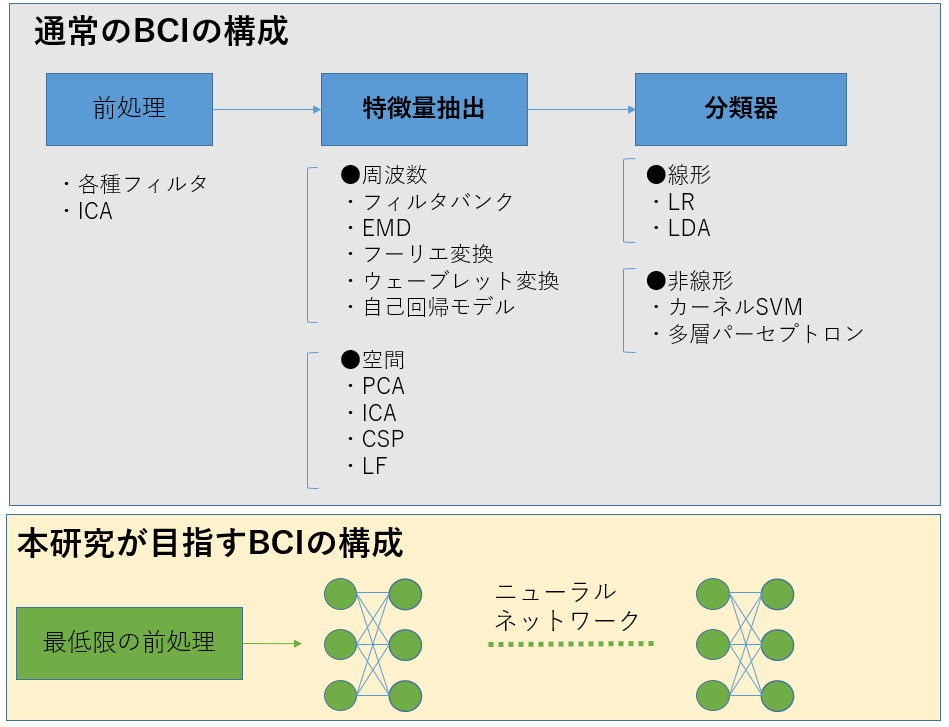
\includegraphics[width=12cm]{images/BCIpattern.PNG}
    \caption{従来のBCIの構成と本研究が目指すBCIの構成}
    \label{fig:BCIpattern}
\end{figure}

またEnd to End学習を提案することによって以下の項目について達成することを目標とした。
\begin{itemize}
    % \item タスク毎のEEGの解析の必要性を排除
    \item 各個人におけるEEGの解析の必要性を排除
    \item 人類に共通した一般的なBCIの可能性を示す
\end{itemize}



% また、ニューラルネットワークの応用研究が盛んな画像認識の分野では、
% 既に模範的なニューラルネットワークの構造が発見されており、
% 大量の画像によって事前学習を行い、
% 達成したい認識対象を絞り込んだ後に転移学習することで
% 手軽に高い性能の分類器が得られる。
% 従って、BCIにおいて模範的なニューラルネットワークの構築により
% 以下の事項が達成できる可能性が示唆される。
% 従って研究の成果によって以下の項目において貢献することができる。

% また、マルチモーダルなBCIの一部としても応用可能である。

% 更に、モデルの構築も含めハイパーパラメータの存在によって
% 試行錯誤の必要性も非常に高い。
% しかし、特徴量抽出手法や分類器自体を変更しながら様々な組み合わせを検討することに比べ、
% ニューラルネットワークの調整は単純作業である。
% また今後ハイパーパラメータの調整自体を自動化する、
% あるいは学習に組み込む方法も出現する可能性がある。


